\documentclass{standalone}
\usepackage{tikz}
\usetikzlibrary{patterns}
\usetikzlibrary{positioning}
\usetikzlibrary{patterns, positioning}
\usetikzlibrary{shapes.misc}
\usepackage[outline]{contour}
\contourlength{1.5pt} 
\usetikzlibrary{calc}
        \usepackage{relsize}
        \tikzset{fontscale/.style = {font=\relsize{#1}}}

\begin{document}
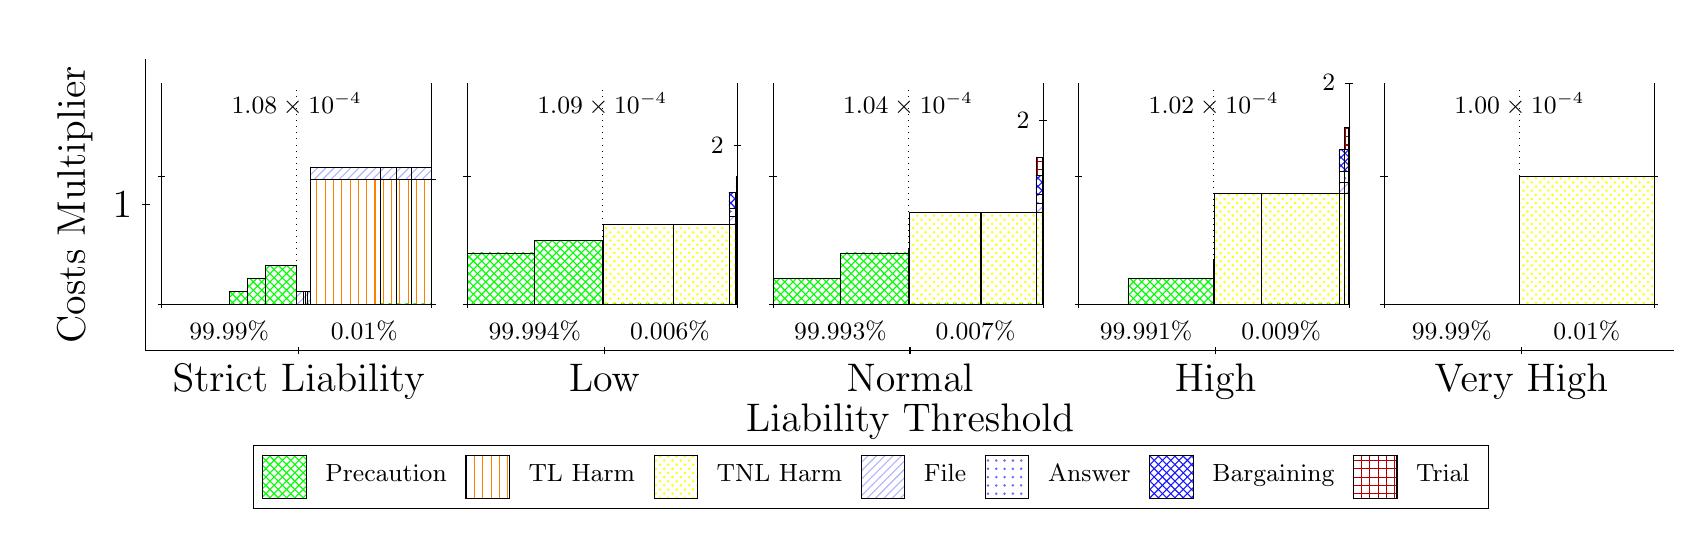
\begin{tikzpicture}
\clip(-0.5,-1.1) rectangle +(20.91,6.2);
\draw[black] (1,1) -- (1,4.7);
\node[rotate=90, fontscale=2, anchor=center] at (0.1, 2.85) {Costs Multiplier};
\draw[black] (0.95,2.85) -- (1.05,2.85);
\node[fontscale=2, anchor=east] at (0.95, 2.85) {1};

\draw[black] (1,1) -- (20.41,1);
\node[fontscale=2, anchor=center] at (10.705, 0.1) {Liability Threshold};
\draw[black] (2.941,0.95) -- (2.941,1.05);
\node[fontscale=2, anchor=north] at (2.941, 0.95) {Strict Liability};
\draw[black] (6.823,0.95) -- (6.823,1.05);
\node[fontscale=2, anchor=north] at (6.823, 0.95) {Low};
\draw[black] (10.705,0.95) -- (10.705,1.05);
\node[fontscale=2, anchor=north] at (10.705, 0.95) {Normal};
\draw[black] (14.587,0.95) -- (14.587,1.05);
\node[fontscale=2, anchor=north] at (14.587, 0.95) {High};
\draw[black] (18.469,0.95) -- (18.469,1.05);
\node[fontscale=2, anchor=north] at (18.469, 0.95) {Very High};


\draw[pattern=crosshatch, pattern color=green,draw=black,very thin] (2.058,1.592) rectangle (2.2894,1.754);
\draw[pattern=crosshatch, pattern color=green,draw=black,very thin] (2.2894,1.592) rectangle (2.5213,1.916);
\draw[pattern=crosshatch, pattern color=green,draw=black,very thin] (2.5213,1.592) rectangle (2.916,2.078);
\draw[pattern=north east lines, pattern color=blue!30,draw=black,very thin] (2.916,1.592) rectangle (3.004,1.7498);
\draw[pattern=crosshatch, pattern color=green,draw=black,very thin] (3.004,1.592) rectangle (3.0278,1.592);
\draw[pattern=north east lines, pattern color=blue!30,draw=black,very thin] (3.004,1.592) rectangle (3.0278,1.7499);
\draw[pattern=crosshatch, pattern color=green,draw=black,very thin] (3.0278,1.592) rectangle (3.0517,1.592);
\draw[pattern=north east lines, pattern color=blue!30,draw=black,very thin] (3.0278,1.592) rectangle (3.0517,1.7499);
\draw[pattern=crosshatch, pattern color=green,draw=black,very thin] (3.0517,1.592) rectangle (3.0923,1.592);
\draw[pattern=north east lines, pattern color=blue!30,draw=black,very thin] (3.0517,1.592) rectangle (3.0923,1.7499);
\draw[pattern=vertical lines, pattern color=orange,draw=black,very thin] (3.0923,1.592) rectangle (3.973,3.1704);
\draw[pattern=north east lines, pattern color=blue!30,draw=black,very thin] (3.0923,3.1704) rectangle (3.973,3.3283);
\draw[pattern=crosshatch, pattern color=green,draw=black,very thin] (3.973,1.592) rectangle (4.1847,1.592);
\draw[pattern=vertical lines, pattern color=orange,draw=black,very thin] (3.973,1.592) rectangle (4.1847,3.1704);
\draw[pattern=north east lines, pattern color=blue!30,draw=black,very thin] (3.973,3.1704) rectangle (4.1847,3.3283);
\draw[pattern=crosshatch, pattern color=green,draw=black,very thin] (4.1847,1.592) rectangle (4.3688,1.592);
\draw[pattern=vertical lines, pattern color=orange,draw=black,very thin] (4.1847,1.592) rectangle (4.3688,3.1705);
\draw[pattern=north east lines, pattern color=blue!30,draw=black,very thin] (4.1847,3.1705) rectangle (4.3688,3.3283);
\draw[pattern=crosshatch, pattern color=green,draw=black,very thin] (4.3688,1.592) rectangle (4.632,1.592);
\draw[pattern=vertical lines, pattern color=orange,draw=black,very thin] (4.3688,1.592) rectangle (4.632,3.1705);
\draw[pattern=north east lines, pattern color=blue!30,draw=black,very thin] (4.3688,3.1705) rectangle (4.632,3.3283);
\node[font=\small,text=black,anchor=north] at (2.916, 4.4) {$1.08\times 10^{-4}$};
\draw[black,very thin] (1.2,1.592) -- (1.2,4.4);
\draw[black,very thin] (1.15,1.592) -- (1.25,1.592);
\node[font=\small,text=black, anchor=west] at (1.15, 1.592) {};
\draw[black,very thin] (1.15,3.2119) -- (1.25,3.2119);
\node[font=\small,text=black, anchor=west] at (1.15, 3.2119) {};

\draw[black,dotted,very thin] (2.916,1.6762) -- (2.916,4.3158);
\draw[black,very thin] (4.632,1.592) -- (4.632,4.4);
\draw[black,very thin] (4.582,1.592) -- (4.682,1.592);
\node[font=\small,text=black, anchor=east] at (4.582, 1.592) {\contour{white}{}};
\draw[black,very thin] (4.582,3.1704) -- (4.682,3.1704);
\node[font=\small,text=black, anchor=east] at (4.582, 3.1704) {\contour{white}{}};

\draw[black,very thin] (1.2,1.592) -- (4.632,1.592);
\draw[black,very thin] (1.2,1.542) -- (1.2,1.642);
\node[font=\small,text=black, anchor=north] at (1.2, 1.542) {};
\draw[black,very thin] (4.632,1.542) -- (4.632,1.642);
\node[font=\small,text=black, anchor=north] at (4.632, 1.542) {};

\node[font=\small,text=black,anchor=south] at (2.058, 0.992) {99.99\%};
\node[font=\small,text=black,anchor=south] at (3.774, 0.992) {0.01\%};

\draw[pattern=crosshatch, pattern color=green,draw=black,very thin] (5.082,1.592) rectangle (5.94,2.24);
\draw[pattern=crosshatch, pattern color=green,draw=black,very thin] (5.94,1.592) rectangle (6.798,2.402);
\draw[pattern=crosshatch, pattern color=green,draw=black,very thin] (6.798,1.592) rectangle (6.8123,1.592);
\draw[pattern=north east lines, pattern color=blue!30,draw=black,very thin] (6.798,1.592) rectangle (6.8123,1.6929);
\draw[pattern=dots,  pattern color=blue!60,draw=black,very thin] (6.798,1.6929) rectangle (6.8123,1.7938);
\draw[pattern=crosshatch,      pattern color=blue!90,draw=black,very thin] (6.798,1.7938) rectangle (6.8123,1.9956);
\draw[pattern=crosshatch, pattern color=green,draw=black,very thin] (6.8123,1.592) rectangle (6.8156,1.592);
\draw[pattern=north east lines, pattern color=blue!30,draw=black,very thin] (6.8123,1.592) rectangle (6.8156,1.6929);
\draw[pattern=dots,  pattern color=blue!60,draw=black,very thin] (6.8123,1.6929) rectangle (6.8156,1.7938);
\draw[pattern=crosshatch,      pattern color=blue!90,draw=black,very thin] (6.8123,1.7938) rectangle (6.8156,1.9956);
\draw[pattern=grid,            pattern color=red!70!black,draw=black,very thin] (6.8123,1.9956) rectangle (6.8156,2.1974);
\draw[pattern=crosshatch, pattern color=green,draw=black,very thin] (6.8156,1.592) rectangle (7.6964,1.592);
\draw[pattern=crosshatch dots, pattern color=yellow,draw=black,very thin] (6.8156,1.592) rectangle (7.6964,2.601);
\draw[pattern=crosshatch, pattern color=green,draw=black,very thin] (7.6964,1.592) rectangle (7.6985,1.592);
\draw[pattern=vertical lines, pattern color=orange,draw=black,very thin] (7.6964,1.592) rectangle (7.6985,2.601);
\draw[pattern=crosshatch, pattern color=green,draw=black,very thin] (7.6985,1.592) rectangle (8.404,1.5921);
\draw[pattern=crosshatch dots, pattern color=yellow,draw=black,very thin] (7.6985,1.5921) rectangle (8.404,2.601);
\draw[pattern=crosshatch, pattern color=green,draw=black,very thin] (8.404,1.592) rectangle (8.4812,1.592);
\draw[pattern=crosshatch dots, pattern color=yellow,draw=black,very thin] (8.404,1.592) rectangle (8.4812,2.601);
\draw[pattern=north east lines, pattern color=blue!30,draw=black,very thin] (8.404,2.601) rectangle (8.4812,2.7019);
\draw[pattern=dots,  pattern color=blue!60,draw=black,very thin] (8.404,2.7019) rectangle (8.4812,2.8028);
\draw[pattern=crosshatch,      pattern color=blue!90,draw=black,very thin] (8.404,2.8028) rectangle (8.4812,3.0046);
\draw[pattern=crosshatch, pattern color=green,draw=black,very thin] (8.4812,1.592) rectangle (8.4935,1.592);
\draw[pattern=vertical lines, pattern color=orange,draw=black,very thin] (8.4812,1.592) rectangle (8.4935,2.601);
\draw[pattern=north east lines, pattern color=blue!30,draw=black,very thin] (8.4812,2.601) rectangle (8.4935,2.7019);
\draw[pattern=dots,  pattern color=blue!60,draw=black,very thin] (8.4812,2.7019) rectangle (8.4935,2.8028);
\draw[pattern=crosshatch,      pattern color=blue!90,draw=black,very thin] (8.4812,2.8028) rectangle (8.4935,3.0046);
\draw[pattern=crosshatch, pattern color=green,draw=black,very thin] (8.4935,1.592) rectangle (8.5118,1.592);
\draw[pattern=crosshatch dots, pattern color=yellow,draw=black,very thin] (8.4935,1.592) rectangle (8.5118,2.601);
\draw[pattern=north east lines, pattern color=blue!30,draw=black,very thin] (8.4935,2.601) rectangle (8.5118,2.7019);
\draw[pattern=dots,  pattern color=blue!60,draw=black,very thin] (8.4935,2.7019) rectangle (8.5118,2.8028);
\draw[pattern=crosshatch,      pattern color=blue!90,draw=black,very thin] (8.4935,2.8028) rectangle (8.5118,3.0046);
\draw[pattern=grid,            pattern color=red!70!black,draw=black,very thin] (8.4935,3.0046) rectangle (8.5118,3.2064);
\draw[pattern=crosshatch, pattern color=green,draw=black,very thin] (8.5118,1.592) rectangle (8.514,1.592);
\draw[pattern=vertical lines, pattern color=orange,draw=black,very thin] (8.5118,1.592) rectangle (8.514,2.601);
\draw[pattern=north east lines, pattern color=blue!30,draw=black,very thin] (8.5118,2.601) rectangle (8.514,2.7019);
\draw[pattern=dots,  pattern color=blue!60,draw=black,very thin] (8.5118,2.7019) rectangle (8.514,2.8028);
\draw[pattern=crosshatch,      pattern color=blue!90,draw=black,very thin] (8.5118,2.8028) rectangle (8.514,3.0046);
\draw[pattern=grid,            pattern color=red!70!black,draw=black,very thin] (8.5118,3.0046) rectangle (8.514,3.2064);
\node[font=\small,text=black,anchor=north] at (6.798, 4.4) {$1.09\times 10^{-4}$};
\draw[black,very thin] (5.082,1.592) -- (5.082,4.4);
\draw[black,very thin] (5.032,1.592) -- (5.132,1.592);
\node[font=\small,text=black, anchor=west] at (5.032, 1.592) {};
\draw[black,very thin] (5.032,3.212) -- (5.132,3.212);
\node[font=\small,text=black, anchor=west] at (5.032, 3.212) {};

\draw[black,dotted,very thin] (6.798,1.6762) -- (6.798,4.3158);
\draw[black,very thin] (8.514,1.592) -- (8.514,4.4);
\draw[black,very thin] (8.464,3.6099) -- (8.564,3.6099);
\node[font=\small,text=black, anchor=east] at (8.464, 3.6099) {\contour{white}{2}};

\draw[black,very thin] (5.082,1.592) -- (8.514,1.592);
\draw[black,very thin] (5.082,1.542) -- (5.082,1.642);
\node[font=\small,text=black, anchor=north] at (5.082, 1.542) {};
\draw[black,very thin] (8.514,1.542) -- (8.514,1.642);
\node[font=\small,text=black, anchor=north] at (8.514, 1.542) {};

\node[font=\small,text=black,anchor=south] at (5.94, 0.992) {99.994\%};
\node[font=\small,text=black,anchor=south] at (7.656, 0.992) {0.006\%};

\draw[pattern=crosshatch, pattern color=green,draw=black,very thin] (8.964,1.592) rectangle (9.822,1.916);
\draw[pattern=crosshatch, pattern color=green,draw=black,very thin] (9.822,1.592) rectangle (10.68,2.24);
\draw[pattern=crosshatch, pattern color=green,draw=black,very thin] (10.68,1.592) rectangle (10.691,1.592);
\draw[pattern=north east lines, pattern color=blue!30,draw=black,very thin] (10.68,1.592) rectangle (10.691,1.7084);
\draw[pattern=dots,  pattern color=blue!60,draw=black,very thin] (10.68,1.7084) rectangle (10.691,1.8247);
\draw[pattern=crosshatch,      pattern color=blue!90,draw=black,very thin] (10.68,1.8247) rectangle (10.691,2.0575);
\draw[pattern=grid,            pattern color=red!70!black,draw=black,very thin] (10.68,2.0575) rectangle (10.691,2.2902);
\draw[pattern=crosshatch, pattern color=green,draw=black,very thin] (10.691,1.592) rectangle (11.601,1.592);
\draw[pattern=crosshatch dots, pattern color=yellow,draw=black,very thin] (10.691,1.592) rectangle (11.601,2.7556);
\draw[pattern=crosshatch, pattern color=green,draw=black,very thin] (11.601,1.592) rectangle (11.606,1.592);
\draw[pattern=vertical lines, pattern color=orange,draw=black,very thin] (11.601,1.592) rectangle (11.606,2.7556);
\draw[pattern=crosshatch, pattern color=green,draw=black,very thin] (11.606,1.592) rectangle (12.305,1.592);
\draw[pattern=crosshatch dots, pattern color=yellow,draw=black,very thin] (11.606,1.592) rectangle (12.305,2.7557);
\draw[pattern=crosshatch, pattern color=green,draw=black,very thin] (12.305,1.592) rectangle (12.381,1.592);
\draw[pattern=crosshatch dots, pattern color=yellow,draw=black,very thin] (12.305,1.592) rectangle (12.381,2.7556);
\draw[pattern=north east lines, pattern color=blue!30,draw=black,very thin] (12.305,2.7556) rectangle (12.381,2.872);
\draw[pattern=dots,  pattern color=blue!60,draw=black,very thin] (12.305,2.872) rectangle (12.381,2.9884);
\draw[pattern=crosshatch,      pattern color=blue!90,draw=black,very thin] (12.305,2.9884) rectangle (12.381,3.2211);
\draw[pattern=grid,            pattern color=red!70!black,draw=black,very thin] (12.305,3.2211) rectangle (12.381,3.4538);
\draw[pattern=crosshatch, pattern color=green,draw=black,very thin] (12.381,1.592) rectangle (12.396,1.592);
\draw[pattern=vertical lines, pattern color=orange,draw=black,very thin] (12.381,1.592) rectangle (12.396,2.7556);
\draw[pattern=north east lines, pattern color=blue!30,draw=black,very thin] (12.381,2.7556) rectangle (12.396,2.872);
\draw[pattern=dots,  pattern color=blue!60,draw=black,very thin] (12.381,2.872) rectangle (12.396,2.9884);
\draw[pattern=crosshatch,      pattern color=blue!90,draw=black,very thin] (12.381,2.9884) rectangle (12.396,3.2211);
\draw[pattern=grid,            pattern color=red!70!black,draw=black,very thin] (12.381,3.2211) rectangle (12.396,3.4538);
\node[font=\small,text=black,anchor=north] at (10.68, 4.4) {$1.04\times 10^{-4}$};
\draw[black,very thin] (8.964,1.592) -- (8.964,4.4);
\draw[black,very thin] (8.914,1.592) -- (9.014,1.592);
\node[font=\small,text=black, anchor=west] at (8.914, 1.592) {};
\draw[black,very thin] (8.914,3.212) -- (9.014,3.212);
\node[font=\small,text=black, anchor=west] at (8.914, 3.212) {};

\draw[black,dotted,very thin] (10.68,1.6762) -- (10.68,4.3158);
\draw[black,very thin] (12.396,1.592) -- (12.396,4.4);
\draw[black,very thin] (12.346,3.9192) -- (12.446,3.9192);
\node[font=\small,text=black, anchor=east] at (12.346, 3.9192) {\contour{white}{2}};

\draw[black,very thin] (8.964,1.592) -- (12.396,1.592);
\draw[black,very thin] (8.964,1.542) -- (8.964,1.642);
\node[font=\small,text=black, anchor=north] at (8.964, 1.542) {};
\draw[black,very thin] (12.396,1.542) -- (12.396,1.642);
\node[font=\small,text=black, anchor=north] at (12.396, 1.542) {};

\node[font=\small,text=black,anchor=south] at (9.822, 0.992) {99.993\%};
\node[font=\small,text=black,anchor=south] at (11.538, 0.992) {0.007\%};

\draw[pattern=crosshatch, pattern color=green,draw=black,very thin] (13.473,1.592) rectangle (14.562,1.916);
\draw[pattern=north east lines, pattern color=blue!30,draw=black,very thin] (14.562,1.592) rectangle (14.569,1.7324);
\draw[pattern=dots,  pattern color=blue!60,draw=black,very thin] (14.562,1.7324) rectangle (14.569,1.8728);
\draw[pattern=crosshatch,      pattern color=blue!90,draw=black,very thin] (14.562,1.8728) rectangle (14.569,2.1536);
\draw[pattern=north east lines, pattern color=blue!30,draw=black,very thin] (14.569,1.592) rectangle (14.575,1.7324);
\draw[pattern=dots,  pattern color=blue!60,draw=black,very thin] (14.569,1.7324) rectangle (14.575,1.8728);
\draw[pattern=crosshatch,      pattern color=blue!90,draw=black,very thin] (14.569,1.8728) rectangle (14.575,2.1536);
\draw[pattern=grid,            pattern color=red!70!black,draw=black,very thin] (14.569,2.1536) rectangle (14.575,2.4344);
\draw[pattern=crosshatch dots, pattern color=yellow,draw=black,very thin] (14.575,1.592) rectangle (15.172,2.996);
\draw[pattern=crosshatch, pattern color=green,draw=black,very thin] (15.172,1.592) rectangle (16.152,1.592);
\draw[pattern=crosshatch dots, pattern color=yellow,draw=black,very thin] (15.172,1.592) rectangle (16.152,2.996);
\draw[pattern=crosshatch dots, pattern color=yellow,draw=black,very thin] (16.152,1.592) rectangle (16.219,2.996);
\draw[pattern=north east lines, pattern color=blue!30,draw=black,very thin] (16.152,2.996) rectangle (16.219,3.1364);
\draw[pattern=dots,  pattern color=blue!60,draw=black,very thin] (16.152,3.1364) rectangle (16.219,3.2768);
\draw[pattern=crosshatch,      pattern color=blue!90,draw=black,very thin] (16.152,3.2768) rectangle (16.219,3.5576);
\draw[pattern=vertical lines, pattern color=orange,draw=black,very thin] (16.219,1.592) rectangle (16.219,2.996);
\draw[pattern=north east lines, pattern color=blue!30,draw=black,very thin] (16.219,2.996) rectangle (16.219,3.1364);
\draw[pattern=dots,  pattern color=blue!60,draw=black,very thin] (16.219,3.1364) rectangle (16.219,3.2768);
\draw[pattern=crosshatch,      pattern color=blue!90,draw=black,very thin] (16.219,3.2768) rectangle (16.219,3.5576);
\draw[pattern=crosshatch dots, pattern color=yellow,draw=black,very thin] (16.219,1.592) rectangle (16.274,2.996);
\draw[pattern=north east lines, pattern color=blue!30,draw=black,very thin] (16.219,2.996) rectangle (16.274,3.1364);
\draw[pattern=dots,  pattern color=blue!60,draw=black,very thin] (16.219,3.1364) rectangle (16.274,3.2768);
\draw[pattern=crosshatch,      pattern color=blue!90,draw=black,very thin] (16.219,3.2768) rectangle (16.274,3.5576);
\draw[pattern=grid,            pattern color=red!70!black,draw=black,very thin] (16.219,3.5576) rectangle (16.274,3.8384);
\draw[pattern=vertical lines, pattern color=orange,draw=black,very thin] (16.274,1.592) rectangle (16.278,2.996);
\draw[pattern=north east lines, pattern color=blue!30,draw=black,very thin] (16.274,2.996) rectangle (16.278,3.1364);
\draw[pattern=dots,  pattern color=blue!60,draw=black,very thin] (16.274,3.1364) rectangle (16.278,3.2768);
\draw[pattern=crosshatch,      pattern color=blue!90,draw=black,very thin] (16.274,3.2768) rectangle (16.278,3.5576);
\draw[pattern=grid,            pattern color=red!70!black,draw=black,very thin] (16.274,3.5576) rectangle (16.278,3.8384);
\node[font=\small,text=black,anchor=north] at (14.562, 4.4) {$1.02\times 10^{-4}$};
\draw[black,very thin] (12.846,1.592) -- (12.846,4.4);
\draw[black,very thin] (12.796,1.592) -- (12.896,1.592);
\node[font=\small,text=black, anchor=west] at (12.796, 1.592) {};
\draw[black,very thin] (12.796,3.212) -- (12.896,3.212);
\node[font=\small,text=black, anchor=west] at (12.796, 3.212) {};

\draw[black,dotted,very thin] (14.562,1.6762) -- (14.562,4.3158);
\draw[black,very thin] (16.278,1.592) -- (16.278,4.4);
\draw[black,very thin] (16.228,4.4) -- (16.328,4.4);
\node[font=\small,text=black, anchor=east] at (16.228, 4.4) {\contour{white}{2}};

\draw[black,very thin] (12.846,1.592) -- (16.278,1.592);
\draw[black,very thin] (12.846,1.542) -- (12.846,1.642);
\node[font=\small,text=black, anchor=north] at (12.846, 1.542) {};
\draw[black,very thin] (16.278,1.542) -- (16.278,1.642);
\node[font=\small,text=black, anchor=north] at (16.278, 1.542) {};

\node[font=\small,text=black,anchor=south] at (13.704, 0.992) {99.991\%};
\node[font=\small,text=black,anchor=south] at (15.42, 0.992) {0.009\%};

\draw[pattern=crosshatch dots, pattern color=yellow,draw=black,very thin] (18.444,1.592) rectangle (20.16,3.2121);
\node[font=\small,text=black,anchor=north] at (18.444, 4.4) {$1.00\times 10^{-4}$};
\draw[black,very thin] (16.728,1.592) -- (16.728,4.4);
\draw[black,very thin] (16.678,1.592) -- (16.778,1.592);
\node[font=\small,text=black, anchor=west] at (16.678, 1.592) {};
\draw[black,very thin] (16.678,3.2119) -- (16.778,3.2119);
\node[font=\small,text=black, anchor=west] at (16.678, 3.2119) {};

\draw[black,dotted,very thin] (18.444,1.6762) -- (18.444,4.3158);
\draw[black,very thin] (20.16,1.592) -- (20.16,4.4);
\draw[black,very thin] (20.11,1.592) -- (20.21,1.592);
\node[font=\small,text=black, anchor=east] at (20.11, 1.592) {\contour{white}{}};
\draw[black,very thin] (20.11,3.2121) -- (20.21,3.2121);
\node[font=\small,text=black, anchor=east] at (20.11, 3.2121) {\contour{white}{}};

\draw[black,very thin] (16.728,1.592) -- (20.16,1.592);
\draw[black,very thin] (16.728,1.542) -- (16.728,1.642);
\node[font=\small,text=black, anchor=north] at (16.728, 1.542) {};
\draw[black,very thin] (20.16,1.542) -- (20.16,1.642);
\node[font=\small,text=black, anchor=north] at (20.16, 1.542) {};

\node[font=\small,text=black,anchor=south] at (17.586, 0.992) {99.99\%};
\node[font=\small,text=black,anchor=south] at (19.302, 0.992) {0.01\%};

\coordinate (LegendAnchor) at (10.205000000000002,0);
\begin{scope}[align=center]
\matrix[scale=0.6,draw=black,below=0.2cm of LegendAnchor,nodes={draw},column sep=0.12cm]{
\node[rectangle,draw,minimum width=0.55cm,minimum height=0.55cm,pattern=crosshatch, pattern color=green]{}; &
        \node[draw=none,font=\small]{Precaution}; &
\node[rectangle,draw,minimum width=0.55cm,minimum height=0.55cm,pattern=vertical lines, pattern color=orange]{}; &
        \node[draw=none,font=\small]{TL Harm}; &
\node[rectangle,draw,minimum width=0.55cm,minimum height=0.55cm,pattern=crosshatch dots, pattern color=yellow]{}; &
        \node[draw=none,font=\small]{TNL Harm}; &
\node[rectangle,draw,minimum width=0.55cm,minimum height=0.55cm,pattern=north east lines, pattern color=blue!30]{}; &
        \node[draw=none,font=\small]{File}; &
\node[rectangle,draw,minimum width=0.55cm,minimum height=0.55cm,pattern=dots, pattern color=blue!60]{}; &
        \node[draw=none,font=\small]{Answer}; &
\node[rectangle,draw,minimum width=0.55cm,minimum height=0.55cm,pattern=crosshatch, pattern color=blue!90]{}; &
        \node[draw=none,font=\small]{Bargaining}; &
\node[rectangle,draw,minimum width=0.55cm,minimum height=0.55cm,pattern=grid, pattern color=red!70!black]{}; &
        \node[draw=none,font=\small]{Trial}; \\
};\end{scope}

\end{tikzpicture}
\end{document}